

The description of \textit{Fuzzy Logic} has been used by Lotfi A. Zadeh for the very first time within his famous published paper "Fuzzy Sets" .

Zadeh defined Fuzzy Logic ' a kind of logic using graded or qualified statements rather than ones that are strictly true or false . The results of fuzzy reasoning are not as definite as those derived by strict logic but they cover a larger field of discourse ' \cite{lotfi}  .

Fuzzy logic doesn't represents the logic that is fuzzy but the idea that all things can be a member of any cluster at least partly member. The idea behind fuzzy logic describes that all transmissions between clusters (memberhsips) are not so strict that you can change memberships just between 0 and 1. There are also soft and mid transitions between 0-1 .

To understand fuzzy logic we ought get into crisp sets too. In short comparision of \textit{Crispt Sets}  and \textit{Fuzzy Sets} both sets are questioning the classical "tall men" problem's memberships according to height of men (See Fig. \ref{fig:comparison})   .

\subsection{Crisp Sets and Fuzzy Sets}

In crisp sets theory a member can be in only one set. For example, for the relationship with the set “A”, the characteristic function gives us 1 (true) if an element named “u” is the member of the set “A” or 0 (false) if an element named “u” is not the member of the set “A” in the crisp logic \cite{Kasabov:1996:FNN:525657}. Hence, this logic cannot represent vague and ambiguous solutions of any paradoxes.

In fuzzy set theory all elements can be definitely true or false and partly true or false. Fuzzy Logic uses the continuum of logical values between 0 and 1 . When you put your height(cm) in Fig.\ref{fig:comparison} you can see that your degree of membership can be fractional and ambiguous .


\begin{figure}[ht]
    \centering
    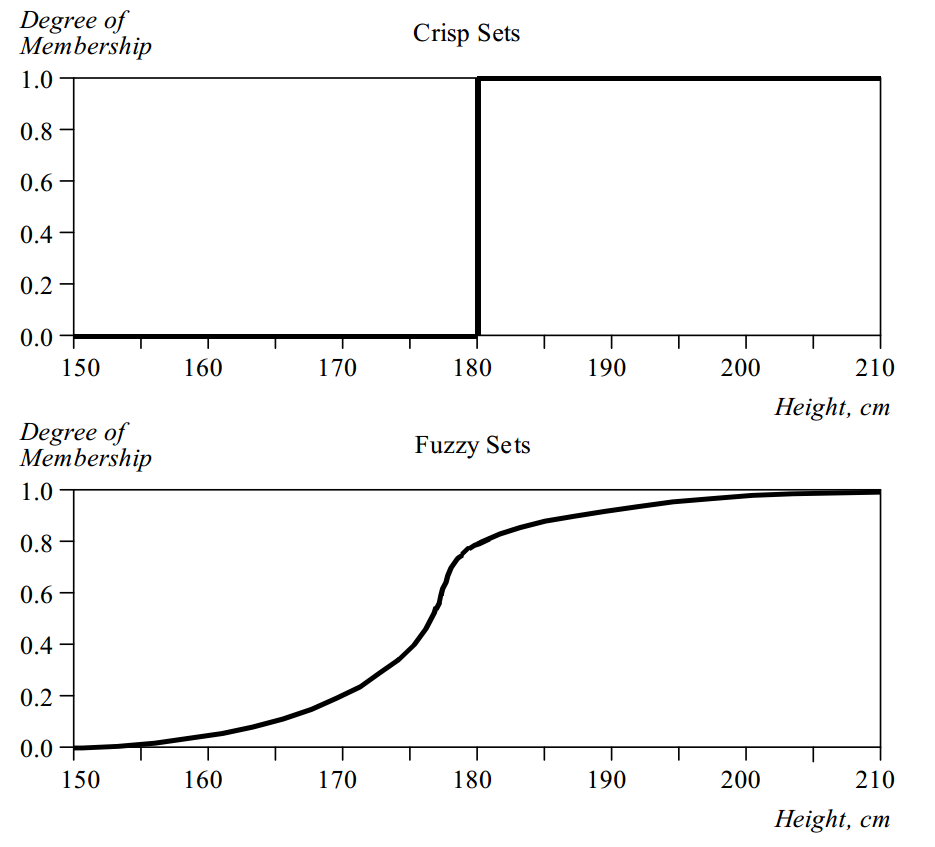
\includegraphics[scale=.3]{Images/crisp_and_fuzzy.png}
    \caption{Crisp and Fuzzy Sets of "\textit{tall men}"}
    \label{fig:comparison}
\end{figure}

\subsection{Fundamentals of Fuzzy Logic} 

Fundamentals of fuzzy decision making can be listed as : Fuzzification , inference and defuzzification.



\textit{1) Fuzzification}


\begin{figure}[ht]
    \centering
    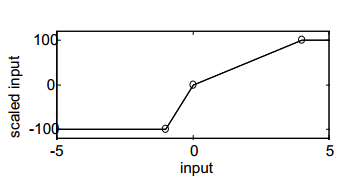
\includegraphics[scale=.55]{Images/fuzzification.png}
    \caption{Example of nonlinear scaling of an input measurement. \cite{jantzen} }
    \label{fig:fig_fuzzification_jantzen}
\end{figure}


Fuzzification explains the process of converting every data to degrees of membership in one or more membership functions. The fuzzificaiton method thus matches the input data with the conditions of the rules . Every data has its own degree of memberships within a fuzzy set which can be explained with a linguistic term .

\textit{2) Inference}

Afterwards of fuzzification an inference is made based on rules . The process which called 'inference' basicly combines all results that evaluated from each rule to obtain a final result. This output given after inference step is also called \textit{fuzzy output set} .


\textit{3) Defuzzification}

After the inference there will be fuzzy output sets. But , its not recognizable in real life . In order to make it usable and recognizable in real life  those values should be translated into real values. This translation named \textit{defuzzification} \cite{defuzzification} .

